\begin{subfigure}[t]{0.45\textwidth}
\centering
\scalebox{0.75}{
 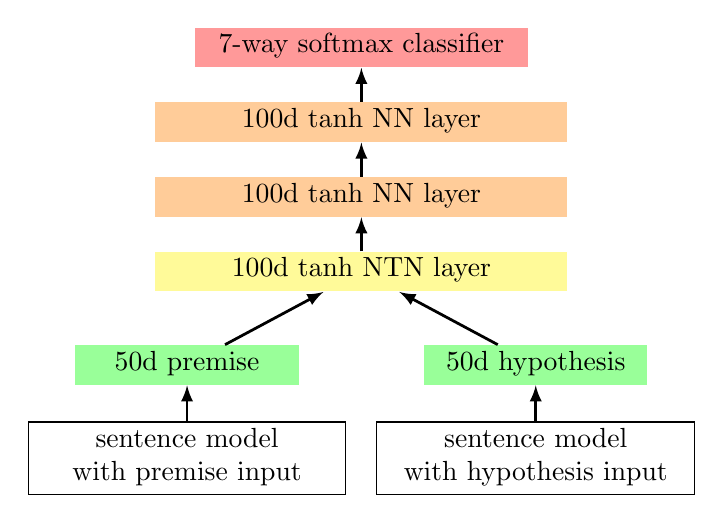
\begin{tikzpicture}
    \def\dx{21pt}
    \def\dy{27pt}

    \tikzstyle{label}=[text width=40mm,align=center,text height=2mm]    
    \tikzstyle{softmax}=[fill=red!40,text width=40mm,align=center,text height=2mm]
    \tikzstyle{preclass}=[fill=orange!40,text width=50mm,align=center,text height=2mm]
    \tikzstyle{e}=[fill=green!40,text width=26mm,align=center,text height=2mm]
    \tikzstyle{m}=[draw=black,text width=38mm,align=center,text height=2mm]    
    
    \node[softmax]  (softmax) at (0*\dx,6*\dy) {7-way softmax classifier};
    \node[preclass]  (pc3) at (0*\dx,5*\dy) {100d $\tanh$ NN layer};
    \node[preclass]  (pc2) at (0*\dx,4*\dy) {100d $\tanh$ NN layer};
    \node[preclass,fill=yellow!40]  (pc1) at (0*\dx,3*\dy) {100d $\tanh$ NTN layer};
    \node[e]  (pe) at (-3*\dx,1.75*\dy) {50d premise};
    \node[e]  (he) at (3*\dx,1.75*\dy) {50d hypothesis};
    \node[m]  (pem) at (-3*\dx,0.5*\dy) {sentence model\\ with premise input};
    \node[m]  (hem) at (3*\dx,0.5*\dy) {sentence model\\ with hypothesis input};    
    
    \pgfsetarrowsend{latex}
    \tikzstyle{fwd} = [draw=black, line width=1pt]

          \draw [fwd] (pc3) -- (softmax);
          \draw [fwd] (pc2) -- (pc3);
          \draw [fwd] (pc1) -- (pc2);
          \draw [fwd] (pe) -- (pc1);
          \draw [fwd] (he) -- (pc1);
          \draw [fwd] (hem) -- (he);
          \draw [fwd] (pem) -- (pe);

  \end{tikzpicture}}
  
 \caption{The general architecture shared across models.}\label{fig:model:top}
  
\end{subfigure}

\begin{subfigure}[t]{0.45\textwidth}
  \centering
\scalebox{0.75}{
 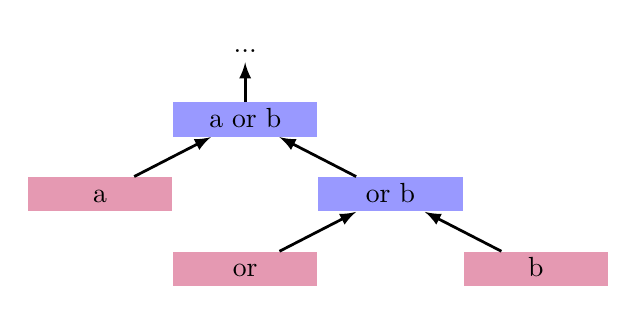
\begin{tikzpicture}
    \def\dx{21pt}
    \def\dy{27pt}


    \tikzstyle{word}=[fill=purple!40,text width=16mm,text height=2mm,align=center]
    \tikzstyle{node}=[fill=blue!40,text width=16mm,text height=2mm,align=center]
    \tikzstyle{empty}=[fill=blue!0,text width=8mm,text height=2mm,align=center]

    \node[empty]  (null) at (0*\dx,7*\dy) {...};
    \node[node]  (aorb) at (0*\dx,6*\dy) {a or b};
    \node[word]  (a) at (-2.5*\dx,5*\dy) {a};
    \node[node]  (orb) at (2.5*\dx,5*\dy) {or b};
    \node[word]  (or) at (0*\dx,4*\dy) {or};
    \node[word]  (b) at (5*\dx,4*\dy) {b};
    
    
    \pgfsetarrowsend{latex}
    \tikzstyle{fwd} = [draw=black, line width=1pt]

          \draw [fwd] (or) -- (orb);
          \draw [fwd] (b) -- (orb);
          \draw [fwd] (a) -- (aorb);
          \draw [fwd] (orb) -- (aorb);
          \draw [fwd] (aorb) -- (null);
  \end{tikzpicture}}
  
     \caption{The architecture for the tree-structured sentence models. Terminal nodes are learned embeddings and nonterminal nodes are NN or NTN layers.}\label{fig:model:tree}
  
  \end{subfigure}
 \vspace{0.5cm}
  
\begin{subfigure}[t]{0.45\textwidth}
  \centering
\scalebox{0.75}{
 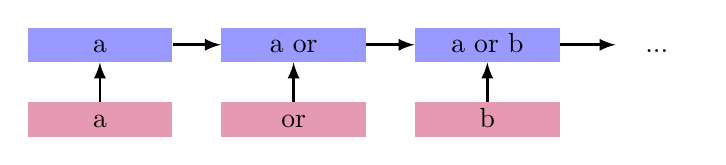
\begin{tikzpicture}
    \def\dx{35pt}
    \def\dy{27pt}


    \tikzstyle{word}=[fill=purple!40,text width=16mm,text height=2mm,align=center]
    \tikzstyle{node}=[fill=blue!40,text width=16mm,text height=2mm,align=center]
    \tikzstyle{empty}=[fill=blue!0,text width=8mm,text height=2mm,align=center]

    \node[word]  (a) at (-3*\dx,1*\dy) {a};
    \node[node]  (aN) at (-3*\dx,2*\dy) {a};
    
    \node[word]  (or) at (-1*\dx,1*\dy) {or};
    \node[node]  (orN) at (-1*\dx,2*\dy) {a or};
    
    \node[word]  (b) at (1*\dx,1*\dy) {b};
    \node[node]  (bN) at (1*\dx,2*\dy) {a or b}; 
    
    \node[empty]  (nullN) at (2.75*\dx,2*\dy) {...}; 
    
    \pgfsetarrowsend{latex}
    \tikzstyle{fwd} = [draw=black, line width=1pt]

          \draw [fwd] (or) -- (orN);
          \draw [fwd] (b) -- (bN);
          \draw [fwd] (a) -- (aN);
          \draw [fwd] (aN) -- (orN);
          \draw [fwd] (orN) -- (bN);
          \draw [fwd] (bN) -- (nullN);
          
  \end{tikzpicture}}
  
   \caption{The architecture for the sequence sentence model. Nodes in the lower row are learned embeddings and nodes on the upper row are LSTM units.}\label{fig:model:seq}
  
    \end{subfigure}